\chapter{Supplemental Figures}

\begin{figure}
  \centering
    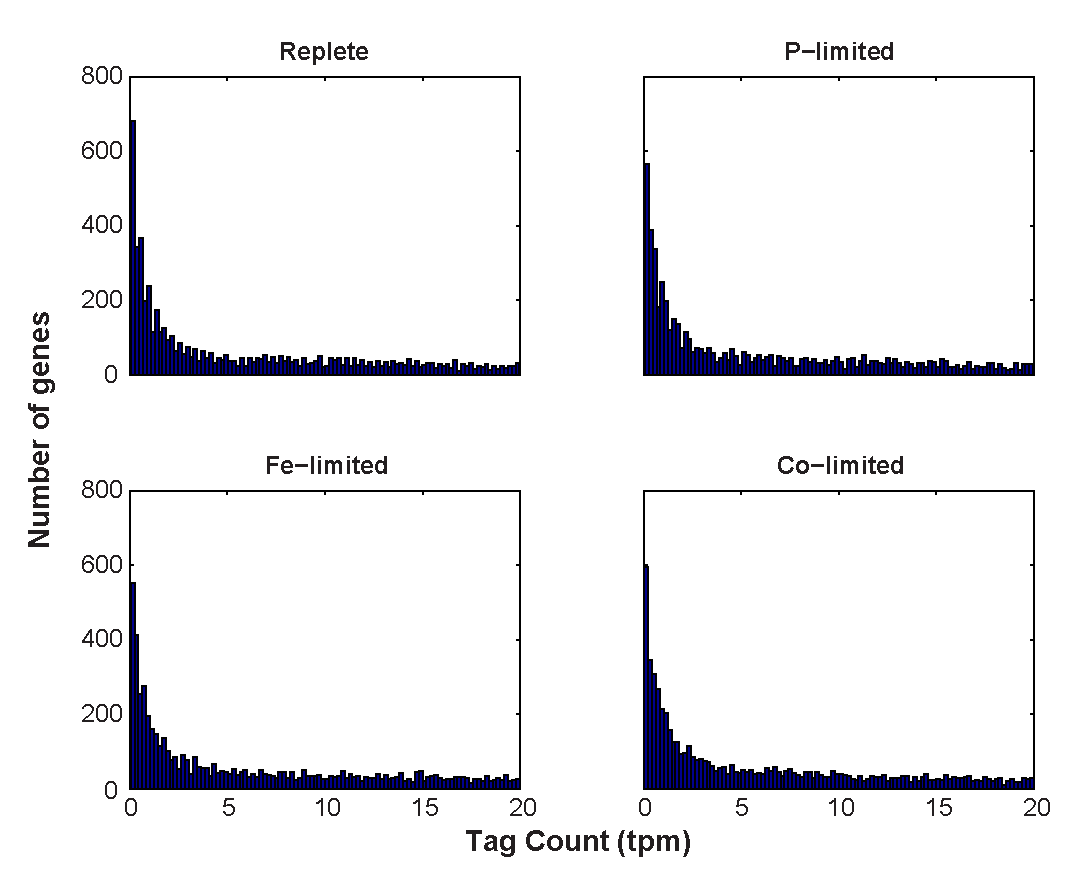
\includegraphics[width=1\textwidth]{Images/C2_FigureS1_v6.pdf}
    \caption[Distribution of normalized tag counts across treatments]{Histogram analysis of the distribution of normalized tag counts (tpm) for each gene across each of the four treatments (Replete, P-limited, Fe-limited, and co-limited). The abundance of normalized tag counts (tpm) was assessed, tallying the total number of genes with a given tag count. Only tag counts less than 20 are depicted to aid the visualization of the inflection in the data at 2.5 tpm.}
  \label{fig:a1f1}
\end{figure}

\begin{landscape}
   \null         %%<---- this is needed
   \vfill        %%<-----here
    
    \begin{figure}
    \centering
        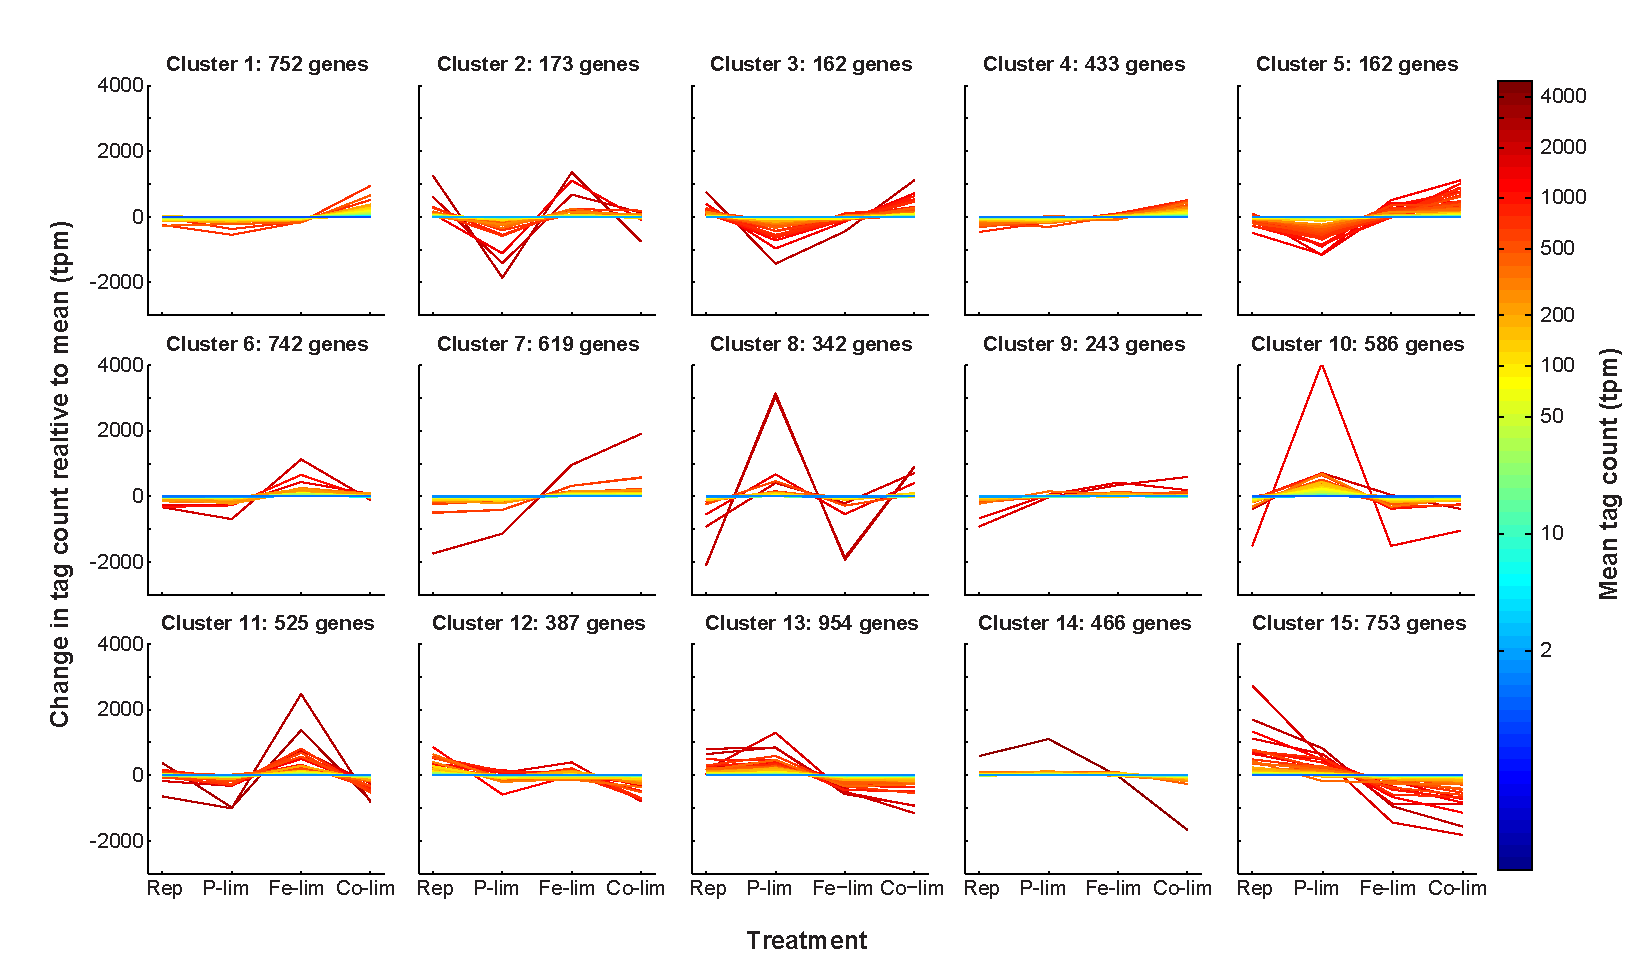
\includegraphics[width=1\textwidth]{Images/C2_FigureS2_v6.pdf}
        \caption[$K$-means clustering of normalized genes]{$K$-means clustering of normalized genes. The 7380 genes that passed the 2.5 tpm cutoff were clustered into 15 clusters using the $k$-means algorithm under the Pearson correlation coefficient. Tag counts normalized to total library size (in tpm) for each gene are plotted relative to the mean (indicated by the color of the line) for each of the four treatments: Replete (Rep), P-limited (P-lim), Fe-limited (Fe-lim), and co-limited (Co-lim).}
    \label{fig:a1f2} 
    \end{figure}
    \vfill        %%<----- and here
\end{landscape}

\clearpage
\newpage
